\section{Grammarware}
\label{sec:grammars-and-metamodels:Grammarware}

In this section, we describe the implementation of our surface language using a tool for text-to-text transformations.
Tools for text-to-text transformations are often referred to as \emph{grammarware}.
We start by describing our approach in Section~\ref{sub:grammars-and-metamodels:GW-Approach}.
Section~\ref{sub:grammars-and-metamodels:GW-Implementation} describes some important aspects of the implementation.

\subsection{Approach}
\label{sub:grammars-and-metamodels:GW-Approach}

\begin{figure}
\centering
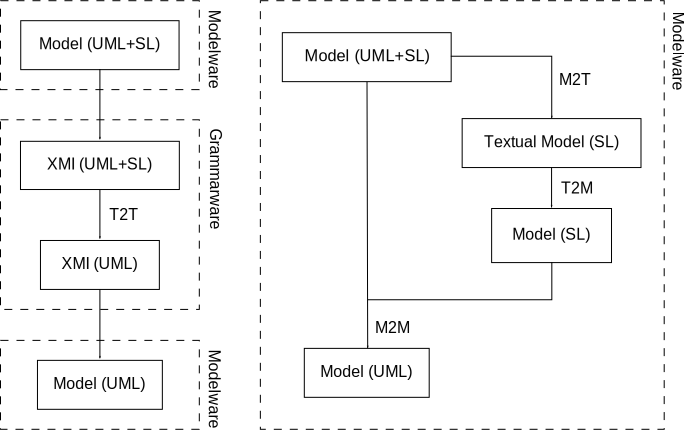
\includegraphics[scale=0.5]{grammars-and-metamodels/figs/approach-comparison}
\caption{Two ways of incorporating textual languages in the UML}
\label{fig:grammars-and-metamodels:approaches}
\end{figure}

The leftmost part of Figure~\ref{fig:grammars-and-metamodels:approaches} gives a schematic overview of the transformation process when performed using a text-to-text (T2T) transformation.
The goal of this process is to transform a \UML model containing behavior specified using a surface language to a plain \UML model.
In the approach using grammarware, we transform models containing fragments of surface language to plain \UML models by transforming the XMI \cite{XMIspec} representations of those models.
This transformation from one textual representation to the other consists of two steps:
\begin{enumerate}
\item A mapping from names occurring in the model to XMI identifiers is made by traversing the parse tree of the XMI representation of the original model and storing each name and the corresponding identifier in a table.
\item The transformation described in Section \ref{sub:grammars-and-metamodels:SL-Transformation} is performed by translating fragments of surface language to XMI representations of equivalent Activities.
\end{enumerate}
The first step of the transformation makes it possible to retrieve the identifier of an element in the second step.
Each element in the XMI representation of a UML model has a unique identifier.
Actions that refer to other elements, such as \AddVariableValueActions and \CreateObjectActions, refer to these other elements using their identifiers.
An \AddVariableValueAction refers to a \Variable using the identifier of that \Variable; a \CreateObjectAction refers to a \Classifier using the identifier of that \Classifier.

Grammarware has been a subject of research for quite some time.
An advantage of using grammarware to perform this transformation is the ease of use provided by the maturity of the tools and their documentation.

A disadvantage of transforming models using a text-to-text transformation is that the models have to be exported to a textual format.
Having to deal with the textual representation of a model lowers the level of abstraction of the transformation.
In our case, for instance, the transformation deals with concepts of the XMI language, at a low level of abstraction, instead of concepts of the \UML, at a higher level of abstraction.


\subsection{Implementation}
\label{sub:grammars-and-metamodels:GW-Implementation}

We implemented the transformation described in Section~\ref{sub:grammars-and-metamodels:SL-Transformation} following the approach described in Section~\ref{sub:grammars-and-metamodels:GW-Approach} in the language \ASFSDF \cite{Deu96.asdf} using an integrated development environment (IDE) for that language, called the \ASFSDFME~\cite{Brand:2001:ASF}.
We discuss some of the details of our implementation below.
The language \ASFSDF and its IDE are described in Appendix~\ref{ap:tools}.

An advantage of using \SDF to define the syntax of our surface language is that it enabled us to combine this definition with an existing syntax definition of the XMI format, without any alterations to the definitions.
This is due to the fact that context-free languages are closed under union.
Because transformations implemented in \ASF are syntax safe, the transformation from \UML models containing fragments of surface language to plain \UML models only produces results that adhere to the definition of XMI.

A disadvantage of the current implementation is that it can only parse one variant of XMI.
Most tools that import or export files in the XMI format use their own interpretation of the format.
These vendor specific interpretations are often incompatible with other interpretations.
Because of this, our implementation is limited to XMI files produced by the UML2 plug-in of Eclipse since it can only read and produce models that adhere to the interpretation of XMI of that plug-in.
A solution for this problem would be to introduce an intermediate language that serves as the starting point of a number of transformations to variants of XMI.
We could then transform a model containing fragments of surface language to this intermediate language and subsequently from this intermediate language to a number of variants of XMI.
The limited portability is another disadvantage of using the Meta-Environment for the implementation of our approach since it is currently only available for the Unix family of operating systems.

Listing~\ref{lst:grammars-and-metamodels:ASF-ex} shows a part of the implementation in \ASF of the transformation from behavior modeled using our surface language to \Activities.
All variable names in this listing start with a dollar sign.
The listing shows that a table mapping names to identifiers, denoted by the variable \ASFVariable{\$Context}, is used both to retrieve the identifier that corresponds to a given name as well as create fresh identifiers.
It also shows that every \ReadVariableAction encountered in a fragment of surface language is replaced by the XMI in lines~7 to~9.

\begin{listing}
  \lstset{
    language=asf,
    style=asf,
    label=lst:grammars-and-metamodels:ASF-ex,
    caption=\ASF rule that creates a \ReadVariableAction,
    numbers=left
  }
  \begin{lstlisting}
    $VariableName := $ReadVariableAction,
    variableExists($Context, $VariableName) == true,
    $Var := getVariableId($Context, $VariableName),
    <$Id1, $Context1> := newId($Context),
    <$Id2, $Context2> := newId($Context1),
    $ObjectContent* :=
    <node xmi:type="uml:ReadVariableAction" xmi:id=$Id1 variable=$Var>
      <result xmi:id=$Id2 />
    </node>
    ====>
    statementWithResult2Action($ReadVariableAction, $Context)=
    <$ObjectContent*, $Id2, $Id1, $Context2>
  \end{lstlisting}
\end{listing}

Listing~\ref{lst:grammars-and-metamodels:An-SDF-definition} shows the part of the \SDF definition that defines the syntax of the surface language statement representing a \ReadVariableAction and declares the corresponding variables.
Line~4 of this definition defines that a \ReadVariableAction is denoted by the name of a variable, as is specified in Section~\ref{sub:grammars-and-metamodels:Syntax-SL}.

\begin{listing}
  \lstset{
    language=sdf,
    label=lst:grammars-and-metamodels:An-SDF-definition,
    caption=\SDF definition that defines the statement representing a \ReadVariableAction,
    numbers=left
  }
  \begin{lstlisting}
    sorts
      ReadVariableAction
    context-free syntax
      VariableName -> ReadVariableAction
    variables
      "$ReadVariableAction"[0-9]* -> ReadVariableAction
  \end{lstlisting}
\end{listing} 